% Dasun's standalone review workspace for issue #67.
% Contains copied Sections 2 and 3 and the layer-table appendix only.
% Build from report/: pdflatex -interaction=nonstopmode -halt-on-error dasun.tex
% Run twice to resolve references. dasun.pdf is a local, ignored review artifact.
% Edit prose here, then copy the marked content back to its canonical section.
% Preamble/styles are copied from main.tex; generated tables/figures stay shared.

\documentclass[11pt]{article}

\usepackage[a4paper,margin=1in]{geometry}
\usepackage{amsmath,amssymb}
\usepackage{graphicx}
\usepackage{xcolor}
\usepackage{listings}
\usepackage{hyperref}
\usepackage{booktabs}
\usepackage{float}
\usepackage{enumitem}
\usepackage{fancyhdr}

% ---------------------------------------------------------------- listings --
% Code styles carried over unchanged from A02.

\definecolor{codebg}{RGB}{234,243,224}
\definecolor{codegreen}{RGB}{0,128,0}
\definecolor{codeblue}{RGB}{0,0,180}
\definecolor{codegray}{RGB}{110,110,110}
\definecolor{codeorange}{RGB}{180,90,0}

\lstdefinestyle{python}{
    backgroundcolor=\color{codebg},
    basicstyle=\ttfamily\footnotesize,
    keywordstyle=\color{codeblue}\bfseries,
    commentstyle=\color{codegray}\itshape,
    stringstyle=\color{codeorange},
    numbers=none,
    breaklines=true,
    breakatwhitespace=false,
    showstringspaces=false,
    frame=single,
    framerule=0pt,
    xleftmargin=2pt,
    xrightmargin=2pt,
    tabsize=4,
    language=Python,
    columns=fullflexible,
    aboveskip=8pt,
    belowskip=8pt
}

\lstdefinestyle{output}{
    backgroundcolor=\color{white},
    basicstyle=\ttfamily\footnotesize,
    frame=single,
    framerule=0.4pt,
    rulecolor=\color{black!40},
    breaklines=true,
    xleftmargin=2pt,
    xrightmargin=2pt,
    aboveskip=4pt,
    belowskip=8pt
}

\lstset{style=python}

\hypersetup{
    colorlinks=true,
    linkcolor=red!70!black,
    urlcolor=blue,
    citecolor=red!70!black
}

\pagestyle{fancy}
\fancyhf{}
\fancyfoot[C]{\thepage}
\renewcommand{\headrulewidth}{0pt}

% ------------------------------------------------------ skeleton helpers --

% Red, bracketed text for anything a human must still fill in. Red so that a
% placeholder left in by accident is impossible to miss in the final PDF;
% #26 (final assembly) must leave none.
\newcommand{\placeholder}[1]{\textcolor{red}{\textbf{[#1]}}}

% A framed note for content an open issue will supply.
\newcommand{\pending}[1]{%
  \begin{center}
  \fbox{\parbox{0.9\linewidth}{\centering\itshape\color{red!70!black}Pending: #1}}%
  \end{center}}

% Generated artifacts that may not exist yet. Each takes the path the
% generator writes to and the issue that produces it. Once the file exists it
% is used as-is; until then the PDF shows where it will go and who owes it.
%   \generatedtable{tables/x.tex}{\#22}
%   \generatedfigure[width=0.8\linewidth]{figures/x.png}{\#22}
% \detokenize prints the path verbatim: generated file names contain
% underscores, which LaTeX would otherwise read as math subscripts.
\newcommand{\generatedtable}[2]{%
  \IfFileExists{#1}{\input{#1}}%
    {\pending{generated table \texttt{\detokenize{#1}} (#2)}}}
\newcommand{\generatedfigure}[3][width=\linewidth]{%
  \IfFileExists{#2}{\includegraphics[#1]{#2}}%
    {\pending{generated figure \texttt{\detokenize{#2}} (#3)}}}

% ------------------------------------------------------------ title data --
% Filled in by #26 (final assembly). The submission file name is
% <groupno>_A03_EN3150.

\newcommand{\groupno}{9}
\newcommand{\repourl}{https://github.com/dpiyumal2319/pattern-recognition-cnn-edge}
% The build date: the submitted PDF is built on submission day.
\newcommand{\submissiondate}{\today}

\title{}
\date{}


\begin{document}
% Personal review workspace for #67. Edit copied prose here before reintegrating.
% BEGIN architecture
\setcounter{section}{1}
\clearpage
\section{Task 2: Custom Architecture Design}
\label{sec:task2}
\subsection{Custom architecture design}
\label{sec:custom-architecture}

Both custom networks take a $64\times64$ RGB image and output ten class
logits.  Each feature-extraction stage has a valid $3\times3$ convolutional
operation with stride~1 and no padding, followed by ReLU and $2\times2$ max
pooling with stride~2.  Because of this, the spatial size goes through
$64\rightarrow62\rightarrow31\rightarrow29\rightarrow14\rightarrow12
\rightarrow6$ over the three stages.  Both networks use channel widths of 32,
64 and 128 and hidden fully connected widths of 128 and 64.  The only
differences are that Model B replaces Model A's standard convolutions with
depthwise separable convolutions, and replaces its flattened head with global
average pooling (GAP).

All convolutional and dense layers have biases, and there is no batch
normalisation in either model.  During training, dropout with probability 0.2
is applied right before each hidden dense layer, and it is turned off for
validation and inference.  The final dense layer outputs raw logits, so there
is no ReLU or softmax after it.

A standard convolution has
\begin{equation}
  P_{\mathrm{conv}}=(K_hK_wC_{\mathrm{in}}+1)C_{\mathrm{out}},
\end{equation}
where the added one is the bias of each output channel.  A depthwise and
pointwise pair instead has
\begin{equation}
  P_{\mathrm{sep}}=(K_hK_w+1)C_{\mathrm{in}}
  +(C_{\mathrm{in}}+1)C_{\mathrm{out}}.
\end{equation}
A dense layer has $(N_{\mathrm{in}}+1)N_{\mathrm{out}}$ parameters.  For one
image, we count convolution MACs as
$K_hK_wC_{\mathrm{in}}C_{\mathrm{out}}H_{\mathrm{out}}W_{\mathrm{out}}$
and dense MACs as $N_{\mathrm{in}}N_{\mathrm{out}}$, and bias additions are
not counted.  Max pooling, ReLU, dropout, flatten and GAP have no trainable
parameters.  Pooling and averaging operations are also left out of the MAC
total, because the project profiler does not count them and the hand
derivation should match the profiler exactly.

\subsubsection{Model A: standard CNN}

Model A flattens the final feature map into $128\times6\times6=4{,}608$
values before the first dense layer, and
Table~\ref{tab:model-a-hand-derivation} derives the parameters and MACs of
every layer from these shapes.

\begin{table}[htbp]
  \centering
  \caption{Hand-derived parameters and MACs for Model A.}
  \label{tab:model-a-hand-derivation}
  \resizebox{\linewidth}{!}{%
  \begin{tabular}{llll}
    \hline
    Layer & Output & Parameter arithmetic & MAC arithmetic \\
    \hline
    Conv 1 & $32\times62\times62$ & $(3\times3\times3+1)\times32=896$
      & $3\times3\times3\times32\times62^2=3{,}321{,}216$ \\
    MaxPool 1 & $32\times31\times31$ & $0$ & $0$ (not profiled) \\
    Conv 2 & $64\times29\times29$ & $(3\times3\times32+1)\times64=18{,}496$
      & $3\times3\times32\times64\times29^2=15{,}501{,}312$ \\
    MaxPool 2 & $64\times14\times14$ & $0$ & $0$ (not profiled) \\
    Conv 3 & $128\times12\times12$ & $(3\times3\times64+1)\times128=73{,}856$
      & $3\times3\times64\times128\times12^2=10{,}616{,}832$ \\
    MaxPool 3 & $128\times6\times6$ & $0$ & $0$ (not profiled) \\
    Flatten & $4{,}608$ & $0$ & $0$ \\
    Dense 1 & $128$ & $(4{,}608+1)\times128=589{,}952$
      & $4{,}608\times128=589{,}824$ \\
    Dense 2 & $64$ & $(128+1)\times64=8{,}256$
      & $128\times64=8{,}192$ \\
    Output & $10$ & $(64+1)\times10=650$ & $64\times10=640$ \\
    \hline
    Total & & $692{,}106$ & $30{,}038{,}016$ \\
    \hline
  \end{tabular}%
  }
\end{table}

The convolutional stack has only $93{,}248$ parameters, while the dense head
has $598{,}858$, which is $86.5\%$ of the total.  So the head is the part that
Model B has to cut if it is to meet its parameter budget.

\subsubsection{Model B: depthwise separable CNN}

In each Model B stage, the depthwise step applies one $3\times3$ filter to
each input channel, and the pointwise $1\times1$ step then mixes those
channels.  There is only one ReLU per stage, and it comes after the pointwise
step.  Table~\ref{tab:model-b-hand-derivation} lists the two convolutions as
separate rows so that the cost of each step can be seen.

\begin{table}[htbp]
  \centering
  \caption{Hand-derived parameters and MACs for Model B. DW and PW denote
  depthwise $3\times3$ and pointwise $1\times1$ convolution.}
  \label{tab:model-b-hand-derivation}
  \resizebox{\linewidth}{!}{%
  \begin{tabular}{llll}
    \hline
    Layer & Output & Parameter arithmetic & MAC arithmetic \\
    \hline
    DW 1 & $3\times62\times62$ & $(3\times3+1)\times3=30$
      & $3\times3\times3\times62^2=103{,}788$ \\
    PW 1 & $32\times62\times62$ & $(3+1)\times32=128$
      & $3\times32\times62^2=369{,}024$ \\
    MaxPool 1 & $32\times31\times31$ & $0$ & $0$ (not profiled) \\
    DW 2 & $32\times29\times29$ & $(3\times3+1)\times32=320$
      & $3\times3\times32\times29^2=242{,}208$ \\
    PW 2 & $64\times29\times29$ & $(32+1)\times64=2{,}112$
      & $32\times64\times29^2=1{,}722{,}368$ \\
    MaxPool 2 & $64\times14\times14$ & $0$ & $0$ (not profiled) \\
    DW 3 & $64\times12\times12$ & $(3\times3+1)\times64=640$
      & $3\times3\times64\times12^2=82{,}944$ \\
    PW 3 & $128\times12\times12$ & $(64+1)\times128=8{,}320$
      & $64\times128\times12^2=1{,}179{,}648$ \\
    MaxPool 3 & $128\times6\times6$ & $0$ & $0$ (not profiled) \\
    GAP and flatten & $128$ & $0$ & $0$ (not profiled) \\
    Dense 1 & $128$ & $(128+1)\times128=16{,}512$
      & $128\times128=16{,}384$ \\
    Dense 2 & $64$ & $(128+1)\times64=8{,}256$
      & $128\times64=8{,}192$ \\
    Output & $10$ & $(64+1)\times10=650$ & $64\times10=640$ \\
    \hline
    Total & & $36{,}968$ & $3{,}725{,}196$ \\
    \hline
  \end{tabular}%
  }
\end{table}

GAP reduces the $128\times6\times6$ tensor to 128 channel means before the
dense stack, so Model B does not need the $4{,}608\rightarrow128$ layer that
dominates Model A.

The separable blocks have $11{,}550$ parameters and the GAP-based dense head
has $25{,}418$, which puts Model B $63{,}032$ parameters below the
100,000-parameter limit.  Keeping a flattened head would leave a
$589{,}952$-parameter first dense layer, and that layer alone is already over
the budget.  Narrowing the channels might also have brought the count under
the limit, but it would reduce the capacity of the feature extractor, so we
used GAP and kept the same channel widths as Model A.

\subsubsection{Compute saving and profiler cross-check}

Table~\ref{tab:separable-mac-saving} compares only the convolution
substitution, at the same input and output shapes.  Over the three stages,
depthwise separable convolution reduces the convolution MACs from
$29{,}439{,}360$ to $3{,}699{,}980$, which is a $7.96\times$ reduction.  The
reduction gets larger as the channel count grows.  For $256\rightarrow256$
channels, the exact cost per output location is
$9\times256\times256=589{,}824$ MACs for a standard convolution and
$9\times256+256\times256=67{,}840$ for the separable version, which gives an
$8.69\times$ reduction.

\begin{table}[htbp]
  \centering
  \caption{Direct MAC comparison between standard and depthwise separable
  convolution at each common stage shape.}
  \label{tab:separable-mac-saving}
  \begin{tabular}{lrrr}
    \hline
    Stage ($C_{\mathrm{in}}\rightarrow C_{\mathrm{out}}$) & Standard & Separable & Reduction \\
    \hline
    $3\rightarrow32$, $62\times62$ & $3{,}321{,}216$ & $472{,}812$ & $7.02\times$ \\
    $32\rightarrow64$, $29\times29$ & $15{,}501{,}312$ & $1{,}964{,}576$ & $7.89\times$ \\
    $64\rightarrow128$, $12\times12$ & $10{,}616{,}832$ & $1{,}262{,}592$ & $8.41\times$ \\
    \hline
    Convolution total & $29{,}439{,}360$ & $3{,}699{,}980$ & $7.96\times$ \\
    \hline
  \end{tabular}
\end{table}

When the classifier heads are included, Model B has $18.72\times$ fewer
trainable parameters and $8.06\times$ fewer MACs per image than Model A,
which are reductions of $94.66\%$ and $87.60\%$.  These are counts and not
measured speedups, because actual inference time also depends on memory
traffic, kernel support and the operations left out of the MAC count.

The forward-hook profiler gives $692{,}106$ parameters and $30{,}038{,}016$
MACs for Model A, and $36{,}968$ parameters and $3{,}725{,}196$ MACs for
Model B.  Both totals agree exactly with the hand derivations, so the tables
describe the networks that we actually trained.

% END architecture
% BEGIN activations
\subsection{Hardware-aware activation-function choice}
\label{sec:activation-choice}

Models A and B use ReLU, $f(x)=\max(0,x)$, after each convolutional stage and
each hidden fully connected layer.  It passes positive values through
unchanged and sets negative values to zero, so it does not saturate for
positive inputs.  The weakness is that negative inputs have zero gradient,
and a unit that stays inactive can stop learning, which is the dying-ReLU
problem.  ReLU outputs are also not zero-centred, which is a second training
risk rather than an inference cost.

Each model applies ReLU to
\begin{equation}
  32(62^2)+64(29^2)+128(12^2)+128+64=195{,}456
\end{equation}
hidden values per image.  Arm's CMSIS-NN Q7 reference implementation compares
each value with zero and sets the negative ones to zero.  On DSP-capable
M-profile cores, its vector path masks four signed 8-bit values in each loop
iteration.\footnote{Arm Ltd., \emph{CMSIS-NN
\texttt{arm\_relu\_q7.c}}, lines 50--101,
\url{https://github.com/ARM-software/CMSIS-NN/blob/71cbe3d5a686c875c88a4d112633b13fae94b5a2/Source/ActivationFunctions/arm_relu_q7.c}.}
The operation needs no coefficients or lookup table.  Loads, stores and loop
control still add to the cycle count, and that count depends on the core and
the compiler.

Sigmoid and tanh, defined as
\begin{equation}
  \sigma(x)=\frac{1}{1+e^{-x}}, \qquad
  \tanh(x)=\frac{e^x-e^{-x}}{e^x+e^{-x}},
\end{equation}
both need exponentials or an approximation of them.  Both functions also
saturate at extreme inputs, where their gradients approach zero.  In CMSIS-NN,
the 16-bit versions of these functions use a 256-entry \texttt{uint16\_t}
sigmoid table.  Inputs inside the table range need two table reads and an
integer interpolation, and inputs outside it take a saturation branch.  The
table takes $256\times2=512$ bytes of read-only memory, before counting code
and temporary values.\footnote{Arm Ltd., \emph{CMSIS-NN
\texttt{arm\_nn\_activation\_s16.c}}, lines 51--117, and
\texttt{arm\_nn\_tables.h}, line 40,
\url{https://github.com/ARM-software/CMSIS-NN/blob/71cbe3d5a686c875c88a4d112633b13fae94b5a2/Source/ActivationFunctions/arm_nn_activation_s16.c},
\url{https://github.com/ARM-software/CMSIS-NN/blob/71cbe3d5a686c875c88a4d112633b13fae94b5a2/Include/arm_nn_tables.h}.}
Using these functions at every hidden site would mean 195,456 such
evaluations per image.  These integer kernels are only examples of embedded
implementations, and our own experiments use the floating-point kernels in
PyTorch.

The cost of floating-point work also depends on the core.  Arm describes the
FPU on Cortex-M4 and Cortex-M7 as optional, and compares hardware floating
point with emulation using integer operations.\footnote{Arm Ltd.,
\emph{DSP capabilities of Cortex-M4 and Cortex-M7}, 2016, pp.~4--5,
\url{https://developer.arm.com/community/arm-community-blogs/b/architectures-and-processors-blog/posts/white-paper-dsp-capabilities-of-cortex-m4-and-cortex-m7}.}
Our activation comparison is therefore analytical, and we did not measure
inference latency on a microcontroller.

GELU's exact form, $x\Phi(x)$, uses the Gaussian cumulative distribution,
which is equivalent to an error function, and its common approximation uses
tanh.\footnote{D. Hendrycks and
K. Gimpel, \emph{Gaussian Error Linear Units (GELUs)}, 2016,
\url{https://arxiv.org/abs/1606.08415}.}
Leaky ReLU and PReLU keep a nonzero gradient on the negative branch when the
slope is nonzero, but they need a multiply on that branch, and PReLU also has
to learn and store the slope $\alpha$.  We chose ReLU because its inference
operation is the simplest of these, but we did not compare the activation
functions experimentally.

\subsubsection{ReLU6 and low-precision deployment}

MobileNetV2 uses
$\operatorname{ReLU6}(x)=\min(\max(0,x),6)$ because a bounded activation holds
up better in low-precision computation.\footnote{M. Sandler et al.,
\emph{MobileNetV2: Inverted Residuals and Linear Bottlenecks}, Section~4,
\url{https://arxiv.org/abs/1801.04381}.}
The upper bound limits the range that has to be represented, so the integer
levels can be spaced more closely inside it.  CMSIS-NN also provides a signed
8-bit ReLU6 operator, but our custom models run in floating point and
quantisation is outside the scope of this project.  We therefore kept ordinary
ReLU, so values above six still reach the next layer.

\subsubsection{Output probabilities}

Softmax converts the ten output logits into normalised probabilities,
\begin{equation}
  p(y=C_k\mid x)=\frac{\exp(z_k)}{\sum_{j=1}^{10}\exp(z_j)}.
\end{equation}
This needs only ten exponentials per image.  Applying an exponential-based
activation to all 195,456 hidden values instead would involve about 19,546
times as many values as the output softmax.

During training, the models return raw logits to \texttt{CrossEntropyLoss}.
At inference, the predicted class is the index of the largest logit, and
softmax does not change this ordering.  Softmax is needed only when normalised
probabilities have to be reported, and on its own it does not make those
probabilities calibrated.

% END activations
\clearpage
% BEGIN optimizer
\section{Task 3: Optimizer Selection and Tuning}
\label{sec:task3}
\subsection{Optimizer comparison protocol}
\label{sec:optimizer-comparison}

We trained Model~B with three optimizer configurations, Adam at
$\alpha=10^{-3}$, plain stochastic gradient descent (SGD) at
$\alpha=10^{-2}$, and SGD at the same learning rate with momentum $m=0.9$.
The model, split manifest, data order and augmentation were the same in every
run.  Each run used seed 42, batch size 128, 30 epochs, zero weight decay and
a fixed learning rate with no scheduler, and the sweep script checks that
these shared settings match before training starts.  The saved Adam
configuration has \texttt{device: auto} while the SGD configurations have
\texttt{device: cuda}, but all three profiles record the same Tesla T4.

SGD updates the weights by
\begin{equation}
  w \leftarrow w-\alpha\frac{\partial L(w)}{\partial w}.
\end{equation}
With momentum, the update becomes
\begin{equation}
  v \leftarrow mv-\alpha\frac{\partial L(w)}{\partial w},
  \qquad w \leftarrow w+v.
\end{equation}
Comparing $m=0$ and $m=0.9$ at the same SGD learning rate therefore isolates
the effect of momentum.  Adam instead scales the step of each parameter using
running first and second moments of the gradients, and we used its default
coefficients $\beta_1=0.9$, $\beta_2=0.999$ and $\epsilon=10^{-8}$.

The learning rates of $10^{-3}$ for Adam and $10^{-2}$ for SGD were starting
values, and we did not run a separate learning-rate search for each optimizer.
Each configuration was also trained with only one seed, so these results
apply to these specific configurations and this training budget rather than
to the optimizers in general.

We selected Adam at $\alpha=10^{-3}$ for the custom-model runs because it
had the lowest validation loss in Table~\ref{tab:optimizer-comparison}.  It
also had the highest validation accuracy at the selected checkpoint and the
highest test accuracy of the three runs.  SGD with momentum reduced
validation loss faster than plain SGD over the 30 epochs.  For every run, the
reported metrics come from the checkpoint with the lowest validation loss,
and test accuracy was used only for the final evaluation.

\begin{table}[htbp]
  \centering
  \small
  \resizebox{\linewidth}{!}{\begin{tabular}{lrrrrrr}
\hline
Optimizer & LR & Momentum & Best val. loss & Best val. acc. (\%) & Test acc. (\%) & Epoch (s) \\
\hline
Adam & 0.001 & 0.0 & 0.427 & 84.42 & 83.75 & 11.61 \\
SGD & 0.01 & 0.0 & 1.996 & 23.14 & 23.48 & 11.12 \\
SGD + momentum & 0.01 & 0.9 & 0.471 & 83.56 & 82.86 & 11.02 \\
\hline
\end{tabular}
}
  \caption{Optimizer comparison for Model~B.  All runs use the same Tesla T4,
  split, seed, data order, batch size, augmentation, and 30-epoch budget.
  Validation accuracy is from the lowest-validation-loss checkpoint, not
  necessarily the maximum-accuracy epoch.  $m$ applies only to SGD, and Adam uses
  its own moment coefficients.  Epoch time is the mean training-pass time,
  excluding validation.}
  \label{tab:optimizer-comparison}
\end{table}

\begin{figure}[H]
  \centering
  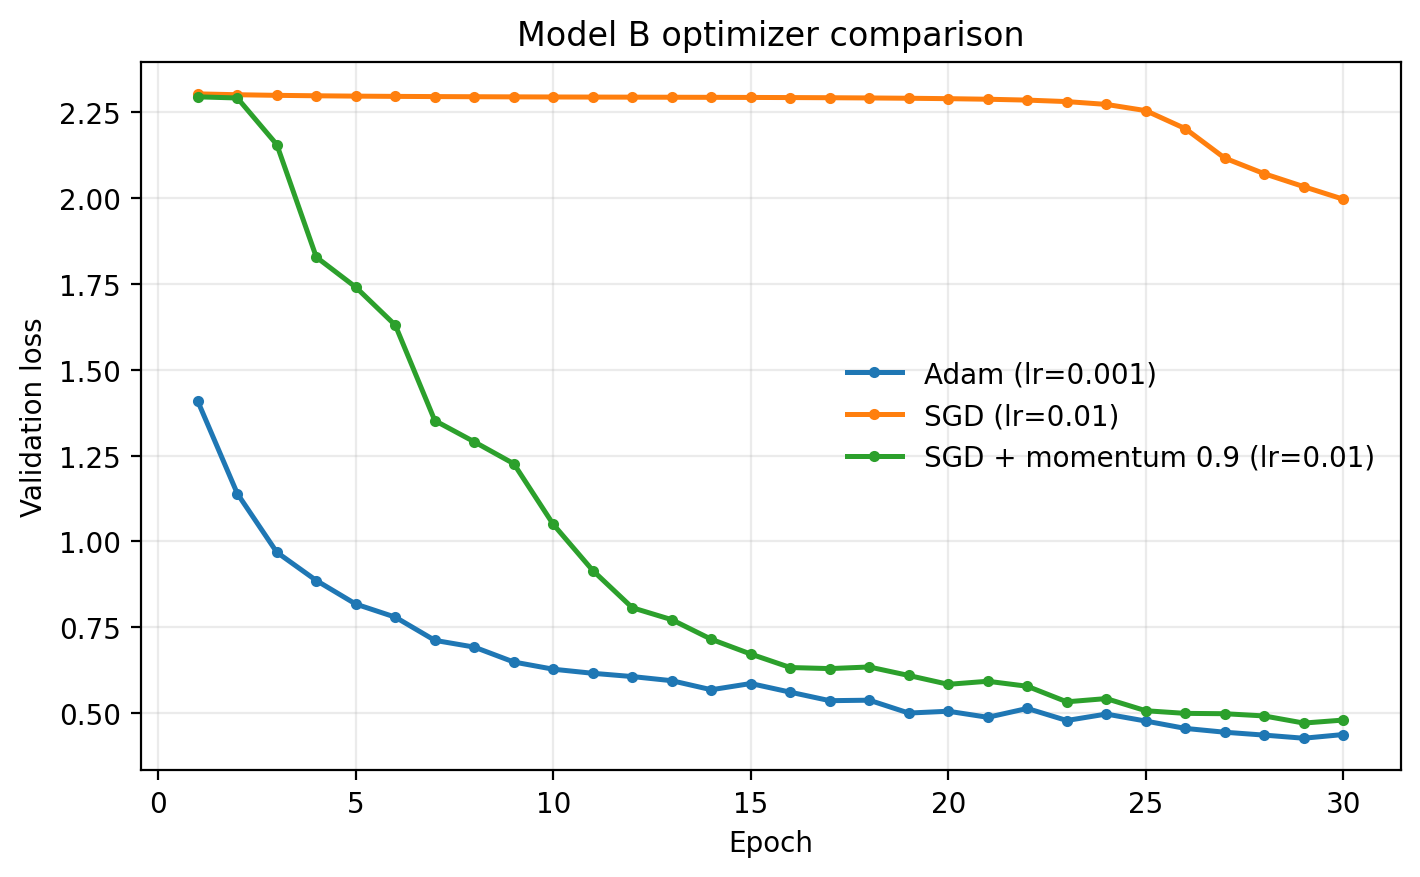
\includegraphics[width=0.86\linewidth]{figures/optimizer_comparison.png}
  \caption{Validation-loss comparison for Adam, plain SGD, and SGD with
  momentum on Model~B under an otherwise identical training budget.}
  \label{fig:optimizer-comparison}
\end{figure}

\subsection{Effect of the momentum coefficient}
\label{sec:momentum-ablation}

We then trained Model~B using SGD with a fixed learning rate of
$\alpha=10^{-2}$ and $m\in\{0,0.5,0.9,0.99\}$.  The split, seed, data order,
augmentation, batch size, initialisation and 30-epoch budget were identical in
all four runs, and all four used an NVIDIA GeForce RTX~3060 Laptop GPU.
Figure~\ref{fig:momentum-ablation} uses the separate
\texttt{momentum\_m000}, \texttt{momentum\_m050}, \texttt{momentum\_m090} and
\texttt{momentum\_m099} records.  Because these ran on a different GPU, their
epoch times cannot be compared directly with the T4 runs in
Table~\ref{tab:optimizer-comparison}.

In the momentum update,
\begin{equation}
  v \leftarrow mv-\alpha\frac{\partial L(w)}{\partial w},
  \qquad w \leftarrow w+v,
  \label{eq:momentum-update}
\end{equation}
$m$ sets how much of the previous velocity is kept.  When successive
gradients have a consistent sign, they accumulate in $v$ and the weights move
further in that direction.  Across a narrow loss ravine, gradient components
that alternate in sign cancel part of the stored velocity, so the side-to-side
motion is damped.

With $m=0$, the update has no memory and validation loss stays high for the
whole epoch budget.  Setting $m=0.5$ makes the loss start falling sooner, but
it is still high after 30 epochs.  The $m=0.9$ run falls with small
epoch-to-epoch fluctuations and reaches the lowest validation loss of the four.
At $m=0.99$ the loss falls fastest at first, but it fluctuates in the later
epochs and finishes above its selected minimum.  Keeping more of the past
velocity could explain these fluctuations, but the saved loss curves do not
record gradient directions, so they cannot show that the updates actually
overshot.

We selected $m=0.9$ because it had the lowest validation loss.  The
$m=0.99$ run had a slightly higher test accuracy, but that did not affect the
choice because test accuracy is not used for selection.  This ranking comes
from one run per setting, and we have not measured whether it holds across
other random seeds.

\begin{figure}[H]
  \centering
  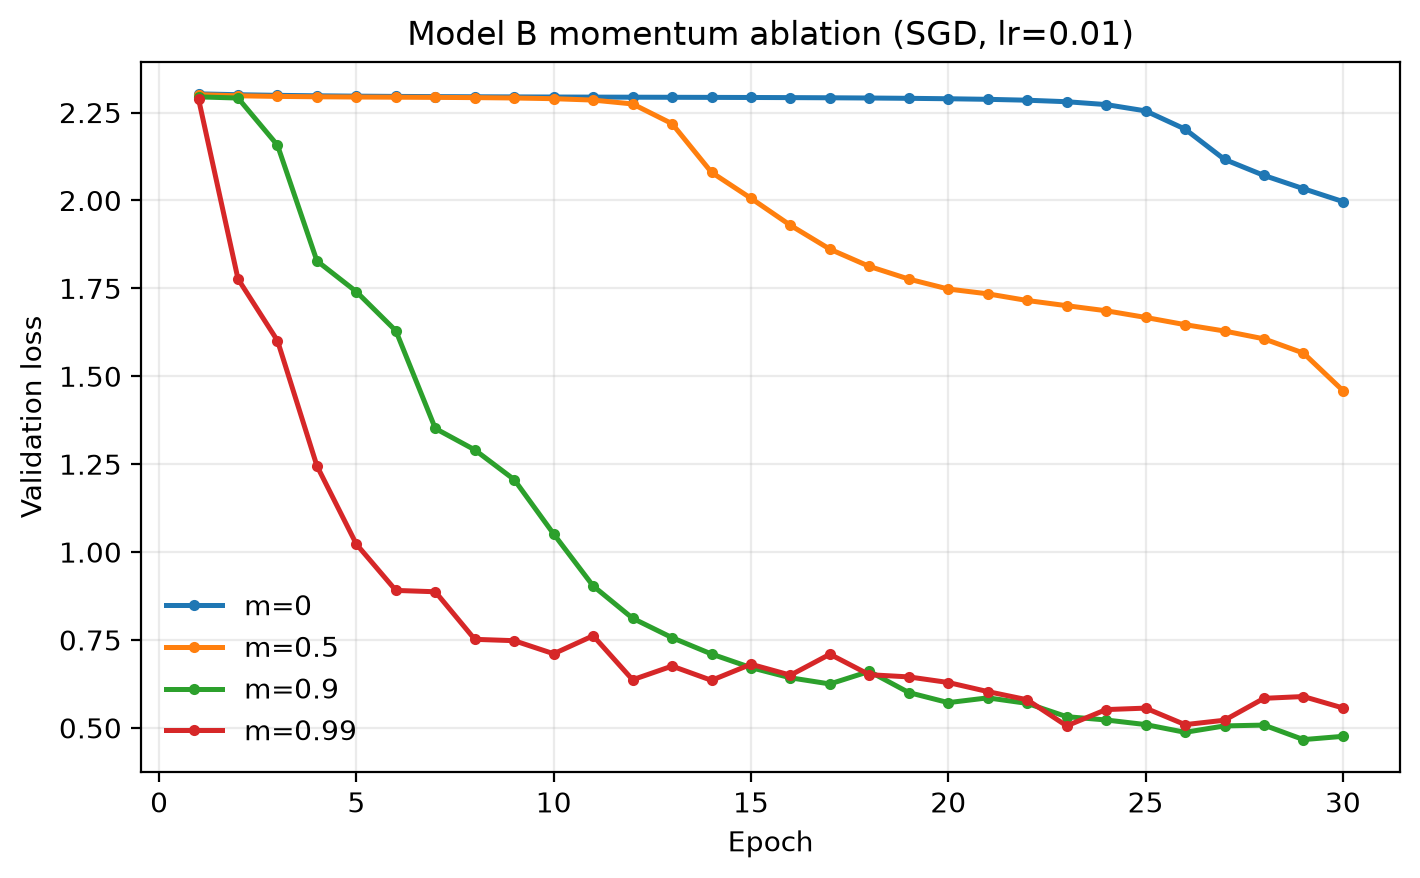
\includegraphics[width=0.86\linewidth]{figures/momentum_ablation.png}
  \caption{Validation-loss curves for Model~B with SGD at
  $\alpha=10^{-2}$.  Momentum is the only methodological variable across the
  four 30-epoch runs.}
  \label{fig:momentum-ablation}
\end{figure}

% END optimizer
\clearpage
% BEGIN appendix
\appendix
\section{Generated Layer Tables}
\label{app:layer-tables}

\texttt{scripts/build\_tables.py} generates these tables from a forward pass
of one $64\times64$ image through each model, and their parameter counts agree
with the hand derivations in Section~\ref{sec:task2}.  The tables only list
operations that change the shape or carry parameters.  ReLU and dropout are
left out of the tables, and their placement is described in
Section~\ref{sec:custom-architecture}.

\begin{table}[H]
  \centering
  \caption{Model A layer summary, generated from \texttt{configs/model\_a.yaml}.}
  \label{tab:model-a-layers}
  \generatedtable{tables/model_a_layers.tex}{\#9}
\end{table}

\begin{table}[H]
  \centering
  \caption{Model B layer summary, generated from \texttt{configs/model\_b.yaml}.
  Each depthwise separable block appears as its two steps.}
  \label{tab:model-b-layers}
  \generatedtable{tables/model_b_layers.tex}{\#10}
\end{table}


% END appendix
\end{document}
